\chapter{Esquema IT}
\section{Análisis del esquema IT}
En este esquema ningún conductor activo debe conectarse directamente a tierra. Además, se debe cumplir que:
\begin{itemize}
	\item La instalación debe tener la fuente
	aislada de tierra o conectada a
	tierra a través de una impedancia
	de valor suficientemente alto
	\item Esta conexión se efectúa desde el
	neutro en caso de estrella o en un
	neutro artificial en caso de triángulo
	\item Si no existe ningún punto de neutro, un
	conductor de fase puede conectarse a
	tierra a través de la impedancia
\end{itemize}
\begin{figure}[H]
	\centering
	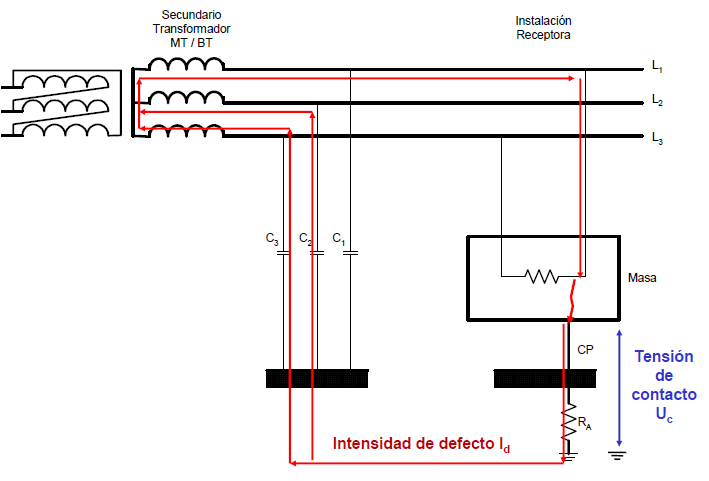
\includegraphics[width=0.7\linewidth]{Images/33}
	\label{fig:33}
\end{figure}

Su circuito equivalente:
\begin{figure}[H]
	\centering
	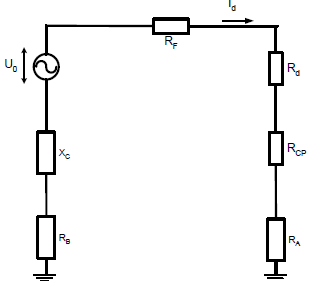
\includegraphics[width=0.4\linewidth]{Images/34}
	\label{fig:34}
\end{figure}

Cuando se da un defecto fase tierra el retorno a tierra se realiza a través de una impedancia muy elevada. Donde la impedancia da aislamiento es:
\begin{equation}
	Z_s\approx X_C= \dfrac{1}{3\omega C_F}
\end{equation}
La corriente de defecto:
\begin{equation}
	I_d=\dfrac{U_F}{Z_S}
\end{equation}

El disparo en caso de defecto no es necesario y se protege contra contactos indirectos con un controlador permanente de aislamiento.

\section{Condiciones de protección primer defecto}
Se debe cumplir que:
\begin{equation}
	R_A\cdot I_d \le U_L
\end{equation}

Como dispositivos de protección se utilizan:
\begin{itemize}
	\item Controlador permanente de aislamiento (CPI)
	\item Interruptores automáticos
	\item Interruptores diferenciales
\end{itemize}

\subsection{Funcionamiento CPI}
\begin{figure}[H]
	\centering
	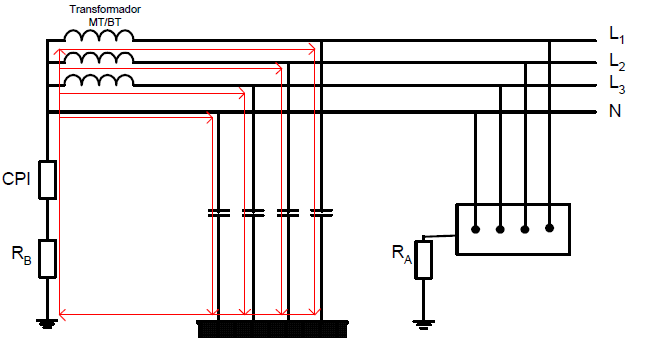
\includegraphics[width=0.7\linewidth]{Images/35}
	\label{fig:35}
\end{figure}

\begin{itemize}
	\item Inyecta aplica una tensión alterna de baja frecuencia entre la red y tierra
	\item Filtro para señal de 50 Hz
	\item Mide la impedancia del aislamiento por la corriente que resulta
\end{itemize}

En caso de fallo:
\begin{figure}[H]
	\centering
	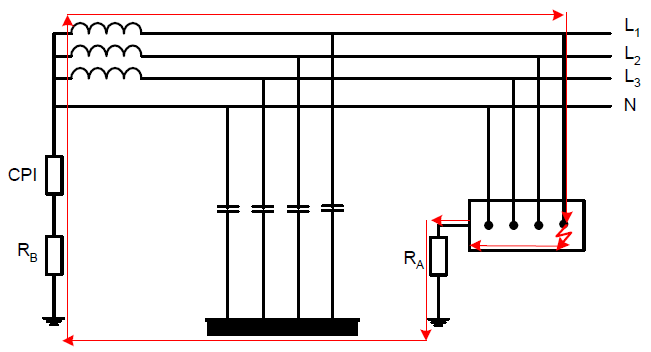
\includegraphics[width=0.7\linewidth]{Images/36}
	\label{fig:36}
\end{figure}

La impedancia vista por el CPI:
\begin{equation}
	Z=\dfrac{1}{4 \omega C}
\end{equation}

Si la impedancia detectada por el CPI es menor avisa del defecto mediante un pitido
\begin{figure}[H]
	\centering
	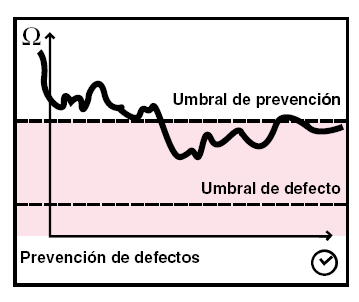
\includegraphics[width=0.4\linewidth]{Images/37}
	\label{fig:37}
\end{figure}

La búsqueda y reparación del primer defecto es esencial para asegurar la
continuidad de servicio que es la propiedad principal del esquema IT
\subsection{Tipos de vigilantes de aislamiento según el principio de funcionamiento}
\begin{itemize}
	\item Pasivos: detectan el defecto de aislamiento a través del desequilibrio de tensiones
	(conexión a todas las fases)
	\item Activos: generan una señal de tensión superpuesta a la de 50 Hz
	\begin{itemize}
		\item Es suficiente con conexión a una parte activa de la
		red, ya que la señal pasa a las otras fases a través
		del bobinado del transformador o del generador. Se
		ponen dos conexiones por seguridad.
	\end{itemize}
\end{itemize}
\subsection{Conexiones CPIs activos en distintos tipos de redes}
\begin{figure}[H]
	\centering
	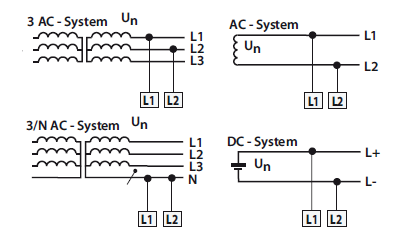
\includegraphics[width=0.6\linewidth]{Images/38}
	\label{fig:38}
\end{figure}

\section{Condiciones de protección doble defecto en distinta fase}
\subsection{Masas puestas a tierra por grupos o individualmente}
\begin{figure}[H]
	\centering
	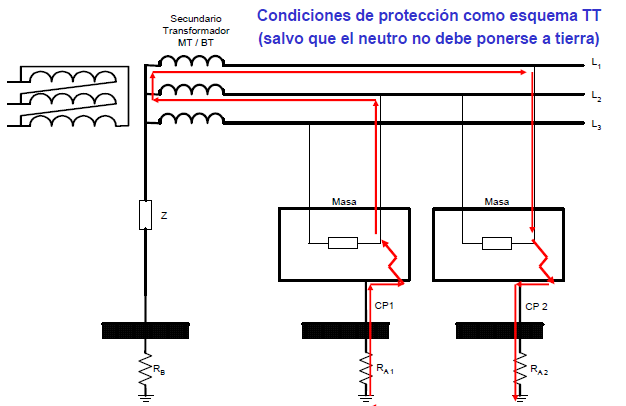
\includegraphics[width=0.5\linewidth]{Images/39}
	\label{fig:39}
\end{figure}

Las condiciones de protección son como en un esquema TT:
\begin{equation}
	R_A\cdot I_{\Delta n} \le U_L
\end{equation}
\subsection{Masas interconectadas entre sí y a tierra y neutro no distribuido}
\begin{figure}[H]
	\centering
	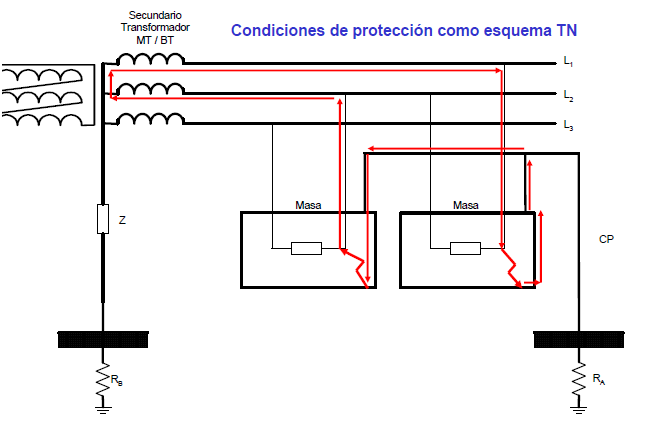
\includegraphics[width=0.5\linewidth]{Images/40}
	\label{fig:40}
\end{figure}

Las condiciones de protección son como en un esquema TN:
\begin{equation}
	2\cdot Z_s\cdot I_{a} \le U_{Linea}
\end{equation}
\subsection{Masas interconectadas entre sí y a tierra y neutro distribuido}
\begin{figure}[H]
	\centering
	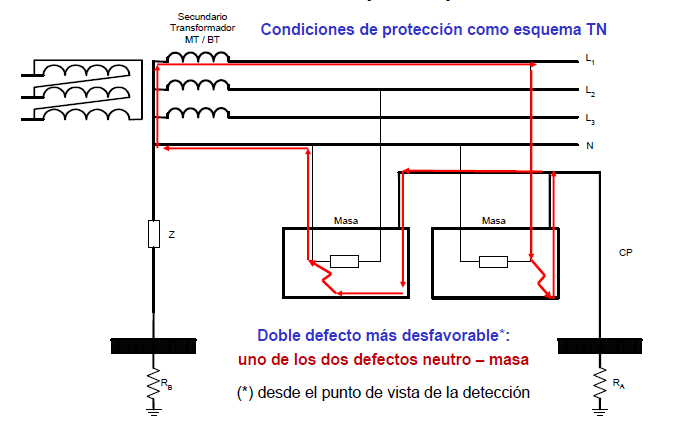
\includegraphics[width=0.5\linewidth]{Images/41}
	\label{fig:41}
\end{figure}
Las condiciones de protección son como en un esquema TN:
\begin{equation}
	2\cdot Z_s\cdot I_{a} \le U_{F}
\end{equation}
\subsection{Resumen de condiciones de protección para doble fallo}
Si no es posible utilizar dispositivos de protección contra
sobreintensidades de forma que se cumplan las condiciones anteriores:
\begin{itemize}
	\item Se utilizarán dispositivos de protección de corriente
	diferencial-residual para cada aparato de utilización
	\item Se realizará una conexión equipotencial complementaria
\end{itemize}
\section{Comparación y selección de esquemas de neutro}

\renewcommand{\arraystretch}{1.5}
\begin{tabular}{|p{3cm}|p{3cm}|p{3cm}|p{5cm}|}
	\hline
	Redes de neutro & TT & TN & IT \\ \hline
	Defecto de aislamiento & 
	Defecto fase-tierra con tierra de retorno & 
	Defecto fase-neutro & 
	Defecto fase-tierra sin tierra de retorno o a través de impedancia de alto valor \\ \hline
	Impedancia bucle de defecto $Z_s$& $R_a+R_B$&$R_F+R_{CP}$&$R_A+C_{FT}$\\ \hline
	Intensidad de defecto $I_d$&$\dfrac{U_0}{Z_s} $&$\dfrac{0,8 U_0}{Z_s} $&$\dfrac{U_0}{Z_s} \approx mA$\\ \hline
	Tensión de contacto $U_c$&$R_A\cdot I_d$&$R_{CP}\cdot I_d$& $R_A\cdot I_d$\\ \hline
	Disparo& Imperativo& Imperativo& No es necesario (aviso y localización)\\ \hline
	Protección contra contactos indirectos& Diferencial donde $I_{\Delta n}\le \dfrac{U_L}{R_A}$& Interruptor automático donde $I_a < I_d$& \begin{itemize}
		\item Primer defecto: señalización por CPI y localización del defecto
		\item Doble defecto:
		\begin{itemize}
			\item Masas no conectadas, red TT
			\item Masas conectadas, red TN
		\end{itemize}
	\end{itemize}\\ \hline
\end{tabular}

\subsection{Selección del esquema de neutro}
Las redes de distribución en baja tensión deben tener esquema TT. Los usuarios que contraten en Alta Tensión podrán elegir, además, el
esquema TN o IT para sus instalaciones de Baja Tensión.
\newline

Los criterios técnicos de selección del esquema de neutro son: 
\begin{itemize}
	\item Seguridad de las personas
	\item Seguridad de las instalaciones
	\item Riesgo de incendio o explosiones
	\item Continuidad de suministro
	\item Compatibilidad electromagnética
	Esquemas
\end{itemize}

\renewcommand{\arraystretch}{1.5}
\begin{center}
\begin{tabular}{|p{3cm}|p{3cm}|p{3cm}|p{3cm}|p{3cm}|}
	\hline
	Redes de neutro & TT & TN-C &TN-S & IT \\ \hline
	Seguridad de personas & Bueno. Protección diferencial obligatoria.&\multicolumn{3}{|p{9cm}|}{ Bueno. Vigilar y garantizar la continuidad del conductor de protección}\\ \hline
	Seguridad de bienes & Bueno&Malo&Malo&Bueno\\ \hline
	Riesgo incendio &Protección diferencia $\le 300 mA$&Malo, corrientes muy altas en el conductor CPN&Protección diferencia $\le 300 mA$& Recomendado para seguridad intrínseca al no producir arco eléctrico\\ \hline
	Riesgo componentes &&No se puede utilizar en locales con riesgo&&\\ \hline
	Disponibilidad energía &Bueno&Bueno&Bueno& Muy bueno\\ \hline
	Comportamiento CEM &\textbf{Bueno}:El conductor de protección deje de ser una referencia de potencial única para la instalación:\begin{itemize}
		\item Instalar pararrayos
		\item Es necesario controlar los equipos con corrientes de fuga elevadas situados después de las protecciones diferenciales
	\end{itemize} &\textbf{Malo}: 
	\begin{itemize}
		\item Circulación de corrientes perturbadoras por las masas.
		\item Relación de perturbaciones por el conductor de protección.
		\item No recomendado si la instalación incluye un generador de armónicos.
	\end{itemize}
	   &\textbf{Muy bueno}:\begin{itemize}
	\item Es necesario controlar los equipos con corrientes de fuga elevadas situados después de las protecciones diferenciales
	\item Corrientes de fallo elevadas en conductor de protección
	\item Una única tierra
	\end{itemize}&\textbf{Malo}: Incompatibilidad con la utilización de filtro en modo común:
	\begin{itemize}
		\item Puede ser necesario fragmentar la instalación para reducir la longitud de los cables y limitar corrientes de fuga
		\item Esquema TN al segundo fallo
	\end{itemize}\\ \hline
\end{tabular}
\end{center}
\subsection{Varios esquemas en una misma instalación}
Es posible alimentar desde un mismo transformador instalaciones con
distinto esquema de neutro, bajo las siguientes condiciones:
\begin{itemize}
	\item Esquemas utilizados sean TN y TT
	\item El conductor CPN de la instalación TN-C conectado al neutro del transformador después
	de su propio dispositivo general de protección
	\item Esquema IT separado de los demás esquemas mediante transformador de aislamiento
	\item Cada instalación con su propio conductor de protección
	\item Cada instalación (edificio o planta) disponga de una red de tierra equipotencial
	\item En esquemas TT e IT las masas y los conductores CP de la misma instalación (edificio o
	planta) se conecten a una misma toma de tierra o varias interconectadas
\end{itemize}